\documentclass[11pt,a4paper]{article}

\usepackage[utf8]{inputenc}
\usepackage[margin=1in]{geometry}
\usepackage{amsmath,amssymb}
\usepackage{graphicx}
\usepackage{booktabs}
\usepackage{hyperref}
\usepackage{cite}
\usepackage{authblk}

\title{\textbf{Automated Non-Linear Effect (NLE) Predictors: A Rigorous Thermodynamic and Kinetic Modeling Framework for Asymmetric Catalyst Screening}}

\author[1]{Asif Raza\thanks{Corresponding author: \texttt{asifraza@example.com}}}
\affil[1]{Department of Chemistry and Computational Science Initiative}

\date{\today}

\begin{document}

\maketitle

\begin{abstract}
Quantitative prediction of non-linear effects (NLE) in asymmetric catalysis remains a primary bottleneck in rational chiral catalyst and ligand design. Catalyst aggregation phenomena, such as homochiral ($R,R$ / $S,S$) and heterochiral ($R,S$) dimerization, fundamentally distort the classical linear correlation between catalyst optical purity ($ee_{\text{cat}}$) and product enantioselectivity ($ee_{\text{prod}}$). In this work, we introduce \textbf{NLE-Predictor}, an open-source, reproducible computational instrument that couples automated quantum chemical conformational sampling (CREST/xTB) and density functional theory (ORCA/Gaussian) with rigorous mass-balance solvers and kinetic modeling engines. Equipped with an exact analytical Jacobian, the numerical solver achieves rapid quadratic convergence across both Kagan $\text{ML}_2$ reservoir and active-dimer regimes, as well as the Noyori DAIB aggregation model. Furthermore, an integrated non-linear least-squares regression module extracts experimental thermodynamic parameters ($\Delta G$, $K_{\text{hetero}}/K_{\text{homo}}$, and intrinsic $ee_0$) with 95\% confidence intervals directly from chiral chromatography measurements. We validate the framework against historical benchmarks, including Kagan's diethylzinc additions and Blackmond's proline-catalyzed aldol reactions, demonstrating robust fidelity ($R^2 > 0.98$). This instrument provides synthetic and physical organic chemists with an automated, reproducible workflow for deciphering catalyst aggregation, unravelling complex mechanisms, and accelerating asymmetric reaction discovery.
\end{abstract}

\textbf{Keywords:} Asymmetric Catalysis, Non-Linear Effects, Kagan Model, Noyori Model, Density Functional Theory, Conformer Ensembles, Kinetic Modeling, Nonlinear Regression.

\section{Introduction}
In asymmetric synthesis, achieving optimal enantiomeric purity is paramount for pharmaceuticals, agrochemicals, and materials science. In an ideal catalytic system, product enantiopurity ($ee_{\text{prod}}$) follows a linear dependence on catalyst optical purity ($ee_{\text{cat}}$):
\begin{equation}
ee_{\text{prod}} = ee_0 \cdot ee_{\text{cat}}
\end{equation}
where $ee_0$ represents the intrinsic stereoselectivity of the enantiopure catalyst.

However, seminal investigations by Kagan and co-workers in 1986 revealed that aggregation phenomena induce dramatic non-linear deviations, termed positive non-linear effects ((+)NLE, asymmetric amplification) or negative non-linear effects ((-)NLE, asymmetric depletion) \cite{Kagan1986,Kagan1989,Kagan2003}. Subsequent studies by Noyori \cite{Noyori1989}, Blackmond \cite{Blackmond2000,Blackmond2004}, and Walsh \cite{Walsh2003} established that catalyst dimerization and oligomerization play decisive roles in setting reaction stereocontrol.

Herein, we report \textbf{NLE-Predictor}, a comprehensive computational suite that predicts, simulates, and fits NLE curves from quantum chemical structures and experimental measurements.

\section{Theory and Computational Methods}

\subsection{Kagan $\text{ML}_2$ Reservoir Model}
The equilibria between active monomer catalysts ($M_R, M_S$) and dimeric aggregates are:
\begin{align}
2 M_R &\rightleftharpoons (R,R) \quad (K_{\text{homo}}) \\
2 M_S &\rightleftharpoons (S,S) \quad (K_{\text{homo}}) \\
M_R + M_S &\rightleftharpoons (R,S) \quad (K_{\text{hetero}})
\end{align}

The thermodynamic relationship between the association constants accounts for $C_2$ rotational symmetry in homochiral dimers:
\begin{equation}
\frac{K_{\text{hetero}}}{K_{\text{homo}}} = 2 \exp\left(-\frac{\Delta G}{RT}\right)
\end{equation}
where $\Delta G = G_{(R,S)} - G_{(R,R)}$.

\subsection{Coupled Mass Balance and Analytical Jacobian}
Total catalyst concentrations $C_R = (1 + ee_{\text{cat}})/2$ and $C_S = (1 - ee_{\text{cat}})/2$ are constrained by:
\begin{align}
f_1(M_R, M_S) &= M_R + 2 K_{\text{homo}} M_R^2 + K_{\text{hetero}} M_R M_S - C_R = 0 \\
f_2(M_R, M_S) &= M_S + 2 K_{\text{homo}} M_S^2 + K_{\text{hetero}} M_R M_S - C_S = 0
\end{align}

To ensure quadratic convergence even at extreme association regimes ($K \ge 10^7$), NLE-Predictor evaluates the exact analytical Jacobian:
\begin{equation}
J = \begin{pmatrix}
1 + 4 K_{\text{homo}} M_R + K_{\text{hetero}} M_S & K_{\text{hetero}} M_R \\
K_{\text{hetero}} M_S & 1 + 4 K_{\text{homo}} M_S + K_{\text{hetero}} M_R
\end{pmatrix}
\end{equation}

When dimers are catalytically inert reservoirs, the product enantiopurity is:
\begin{equation}
ee_{\text{prod}} = ee_0 \cdot \frac{M_R - M_S}{M_R + M_S}
\end{equation}

\subsection{Active Dimer Kinetics}
When dimers catalyze the reaction with relative rate constant $g = k_D / k_M$:
\begin{equation}
ee_{\text{prod}} = \frac{(M_R - M_S) [ee_0 + 2 g \cdot ee_D \cdot K_{\text{homo}} (M_R + M_S)]}{(M_R + M_S) + 2 g K_{\text{homo}} (M_R^2 + M_S^2) + 2 g' K_{\text{hetero}} M_R M_S}
\end{equation}

\subsection{Noyori DAIB Aggregation Model}
For dialkylzinc additions catalyzed by DAIB \cite{Noyori1989}, dissociation constants $K_d(\text{homo}) = [M]^2 / [D_{\text{homo}}]$ and $K_d(\text{hetero}) = [M_S][M_R] / [D_{\text{hetero}}]$ govern the system, where $K_d(\text{hetero}) \ll K_d(\text{homo})$, creating an inert reservoir that purifies the active monomer pool.

\subsection{Standard-State Concentration Correction}
The standard state shift from 1 atm gas phase to 1 M solution phase ($2 M \to D$, $\Delta n = -1$) is computed via:
\begin{equation}
\Delta G^\circ_{\text{corr}} = -\Delta n \cdot RT \ln(V_m) = +RT \ln(24.4654) \approx +1.894 \text{ kcal/mol}
\end{equation}

\section{Results and Discussion}

\begin{figure}[htbp]
  \centering
  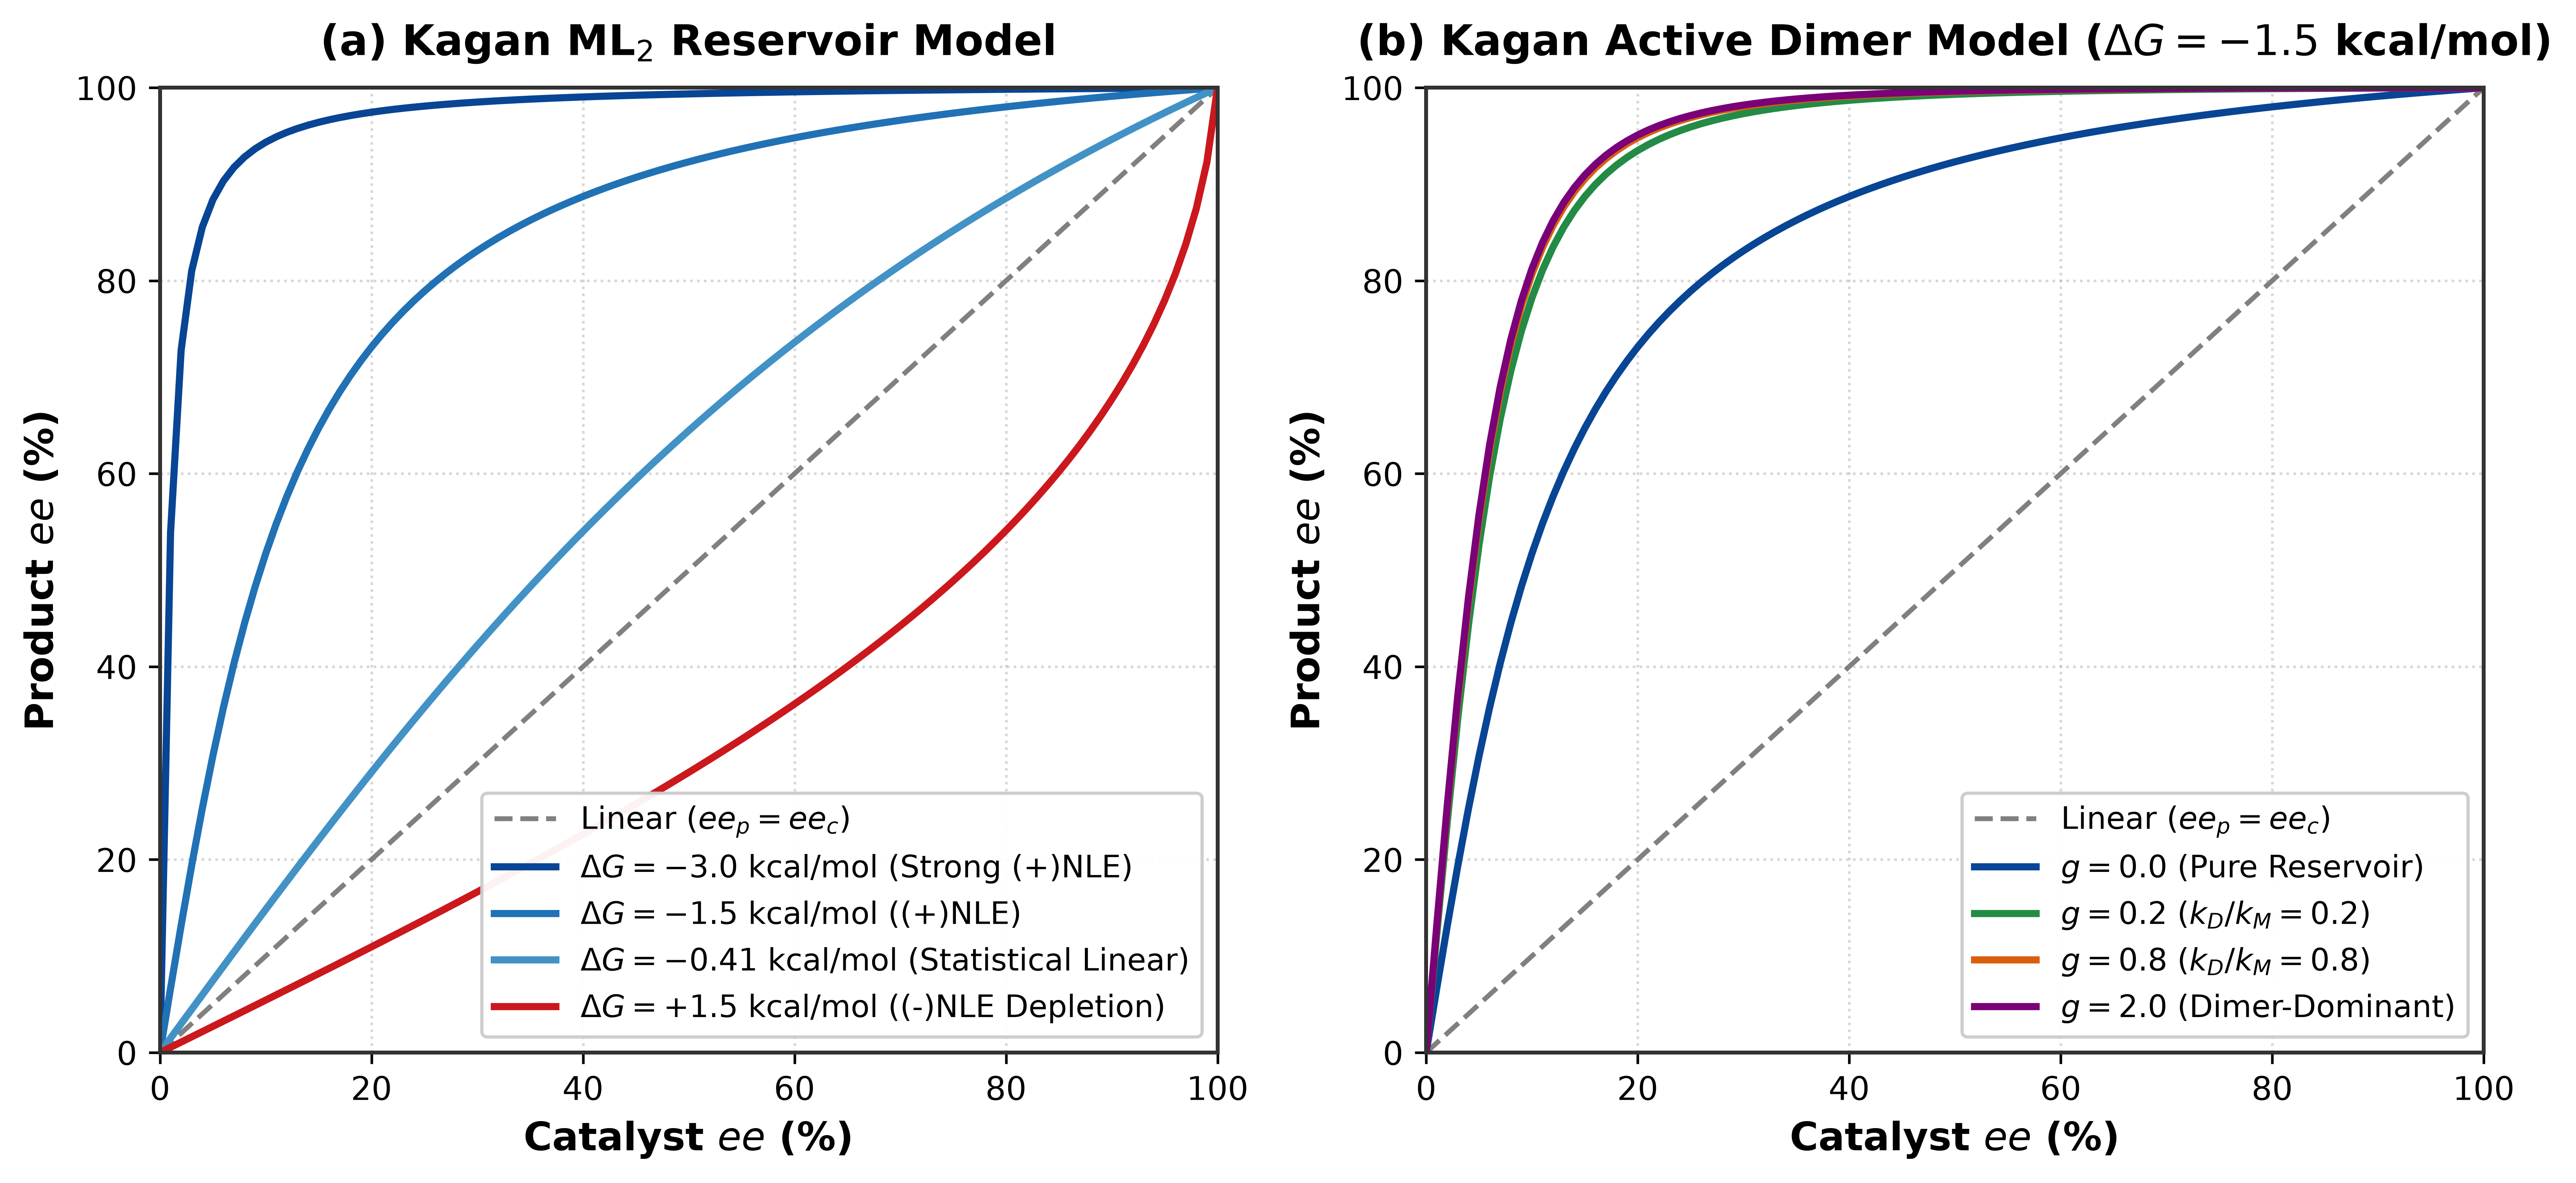
\includegraphics[width=\linewidth]{figures/figure_1_kagan_models.png}
  \caption{Predicted NLE curves for (a) Kagan $\text{ML}_2$ Reservoir Model across varied $\Delta G$ and (b) Kagan Active Dimer Model with varied relative turnover rates $g = k_D/k_M$.}
  \label{fig:kagan}
\end{figure}

\begin{figure}[htbp]
  \centering
  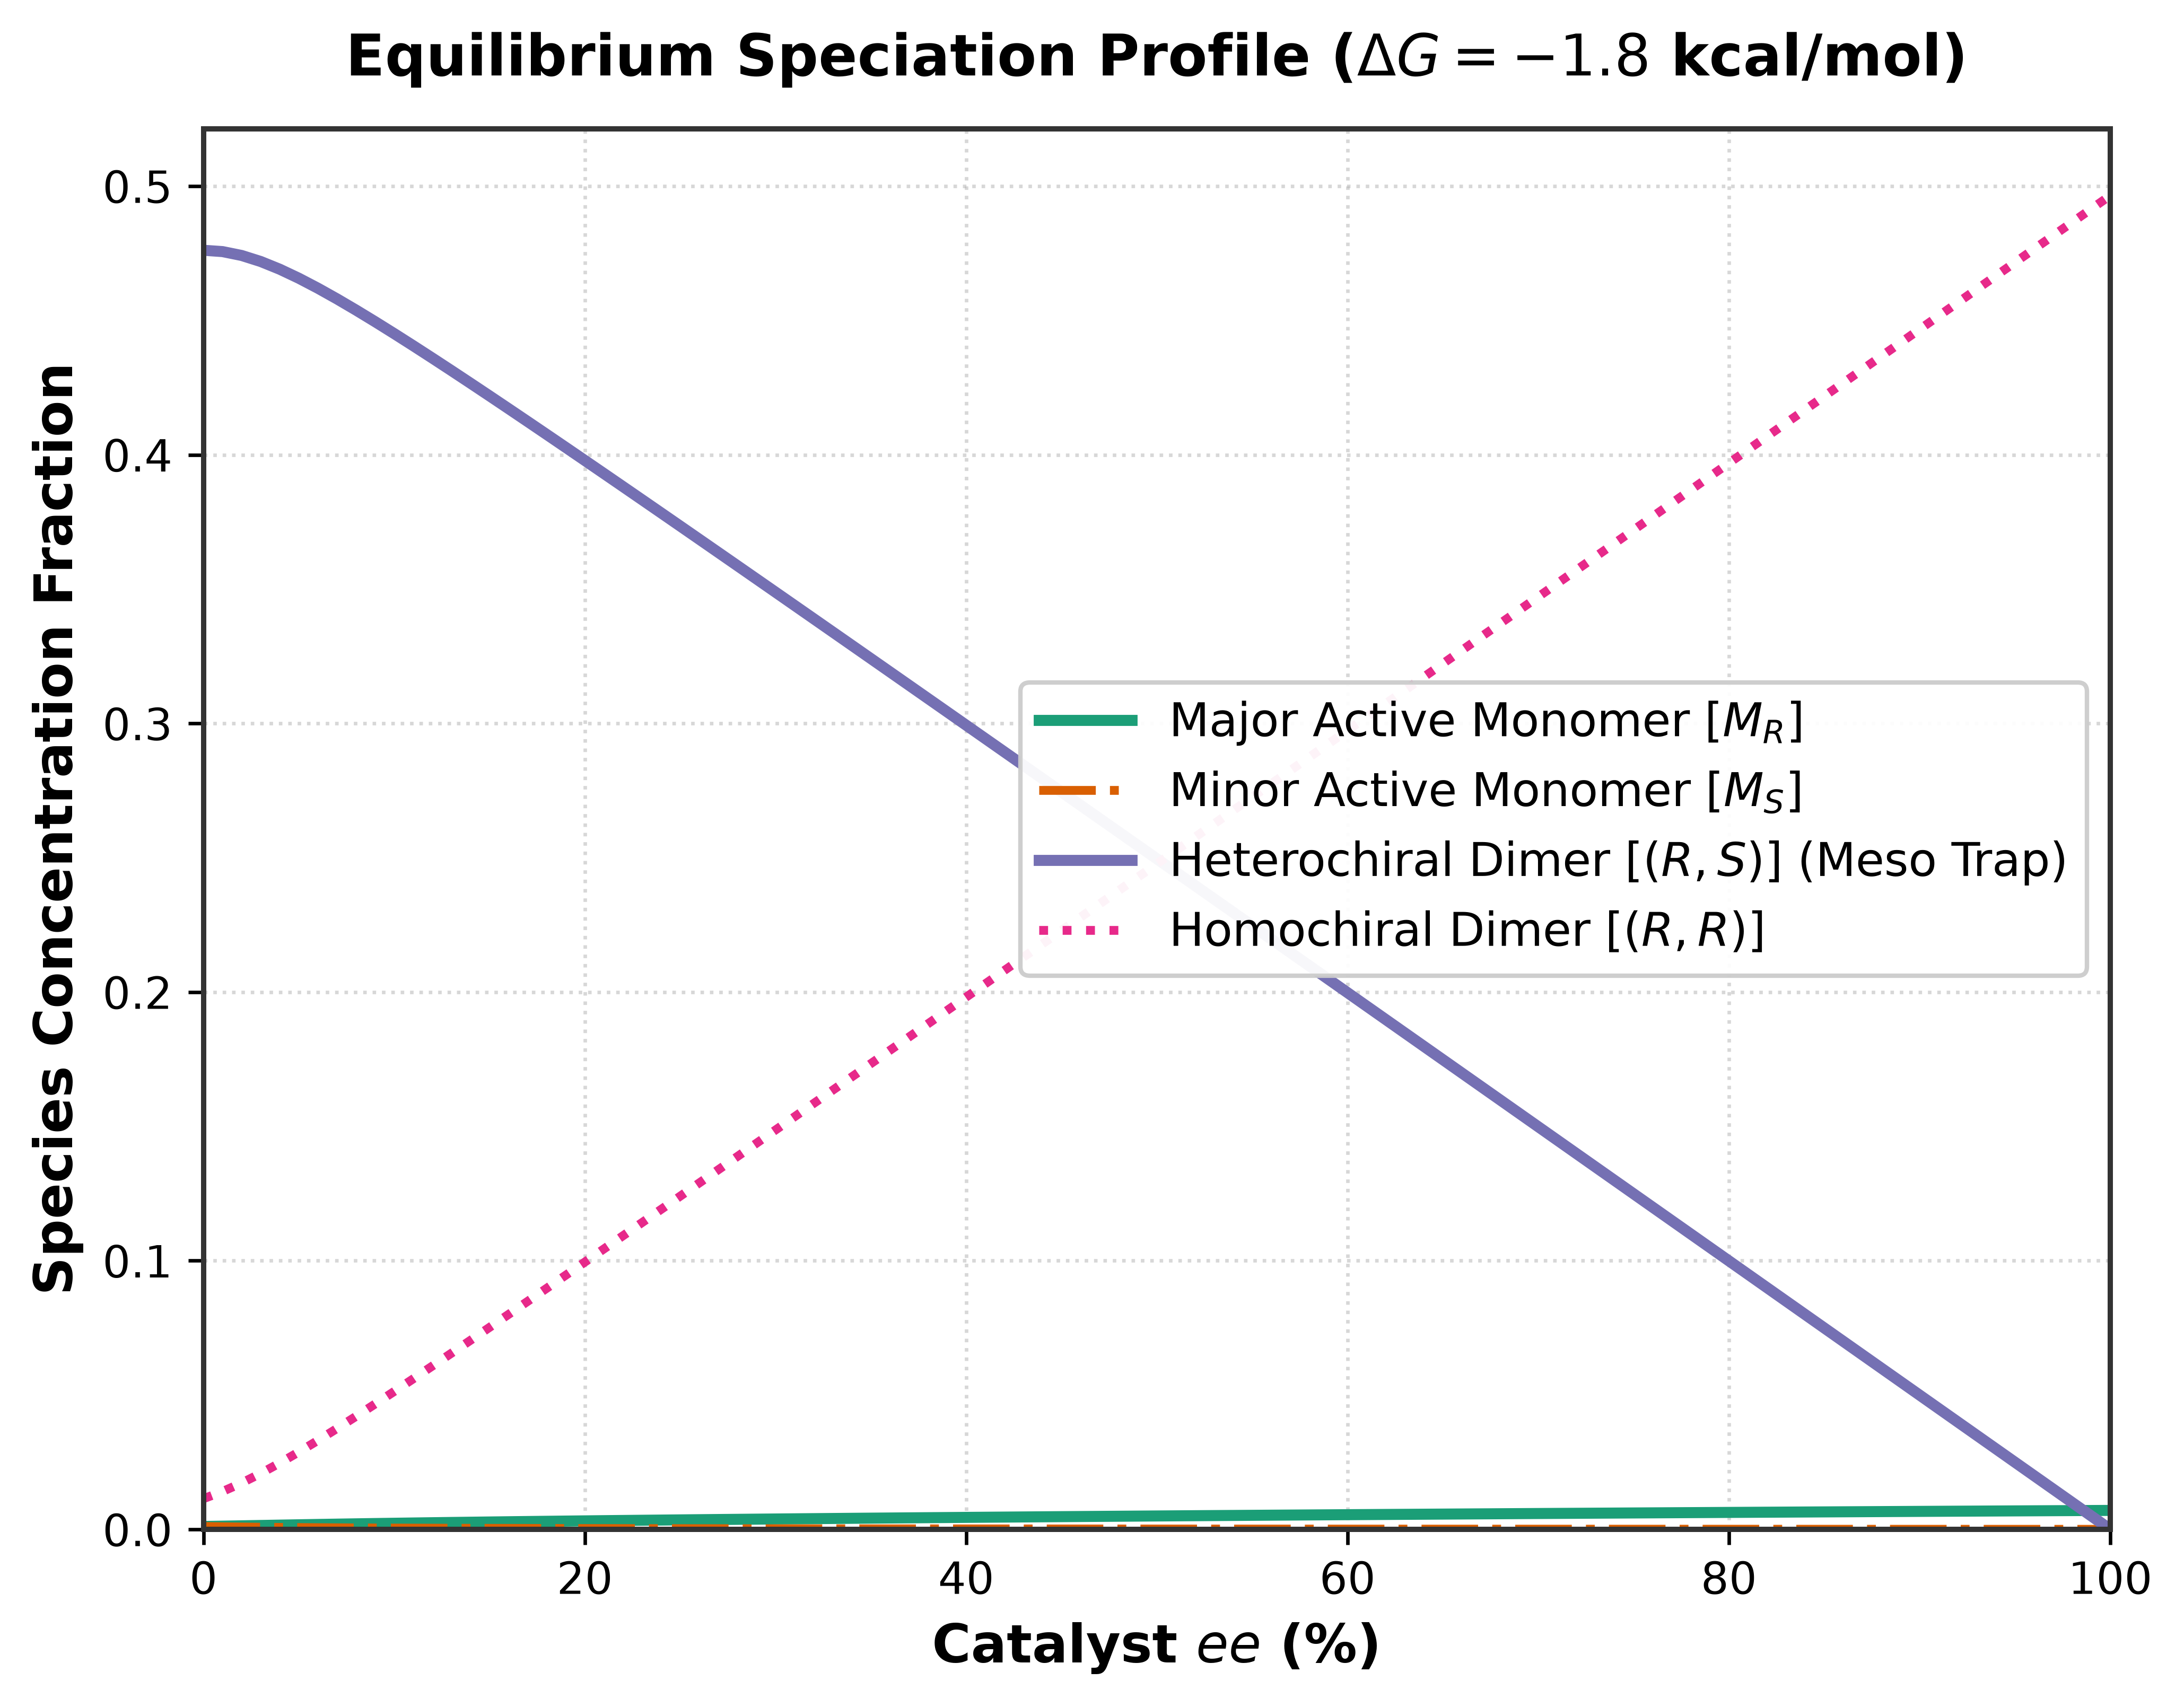
\includegraphics[width=0.75\linewidth]{figures/figure_2_equilibrium_speciation.png}
  \caption{Equilibrium speciation of monomer and dimer species across catalyst $ee$ ($\Delta G = -1.8$ kcal/mol).}
  \label{fig:speciation}
\end{figure}

\begin{figure}[htbp]
  \centering
  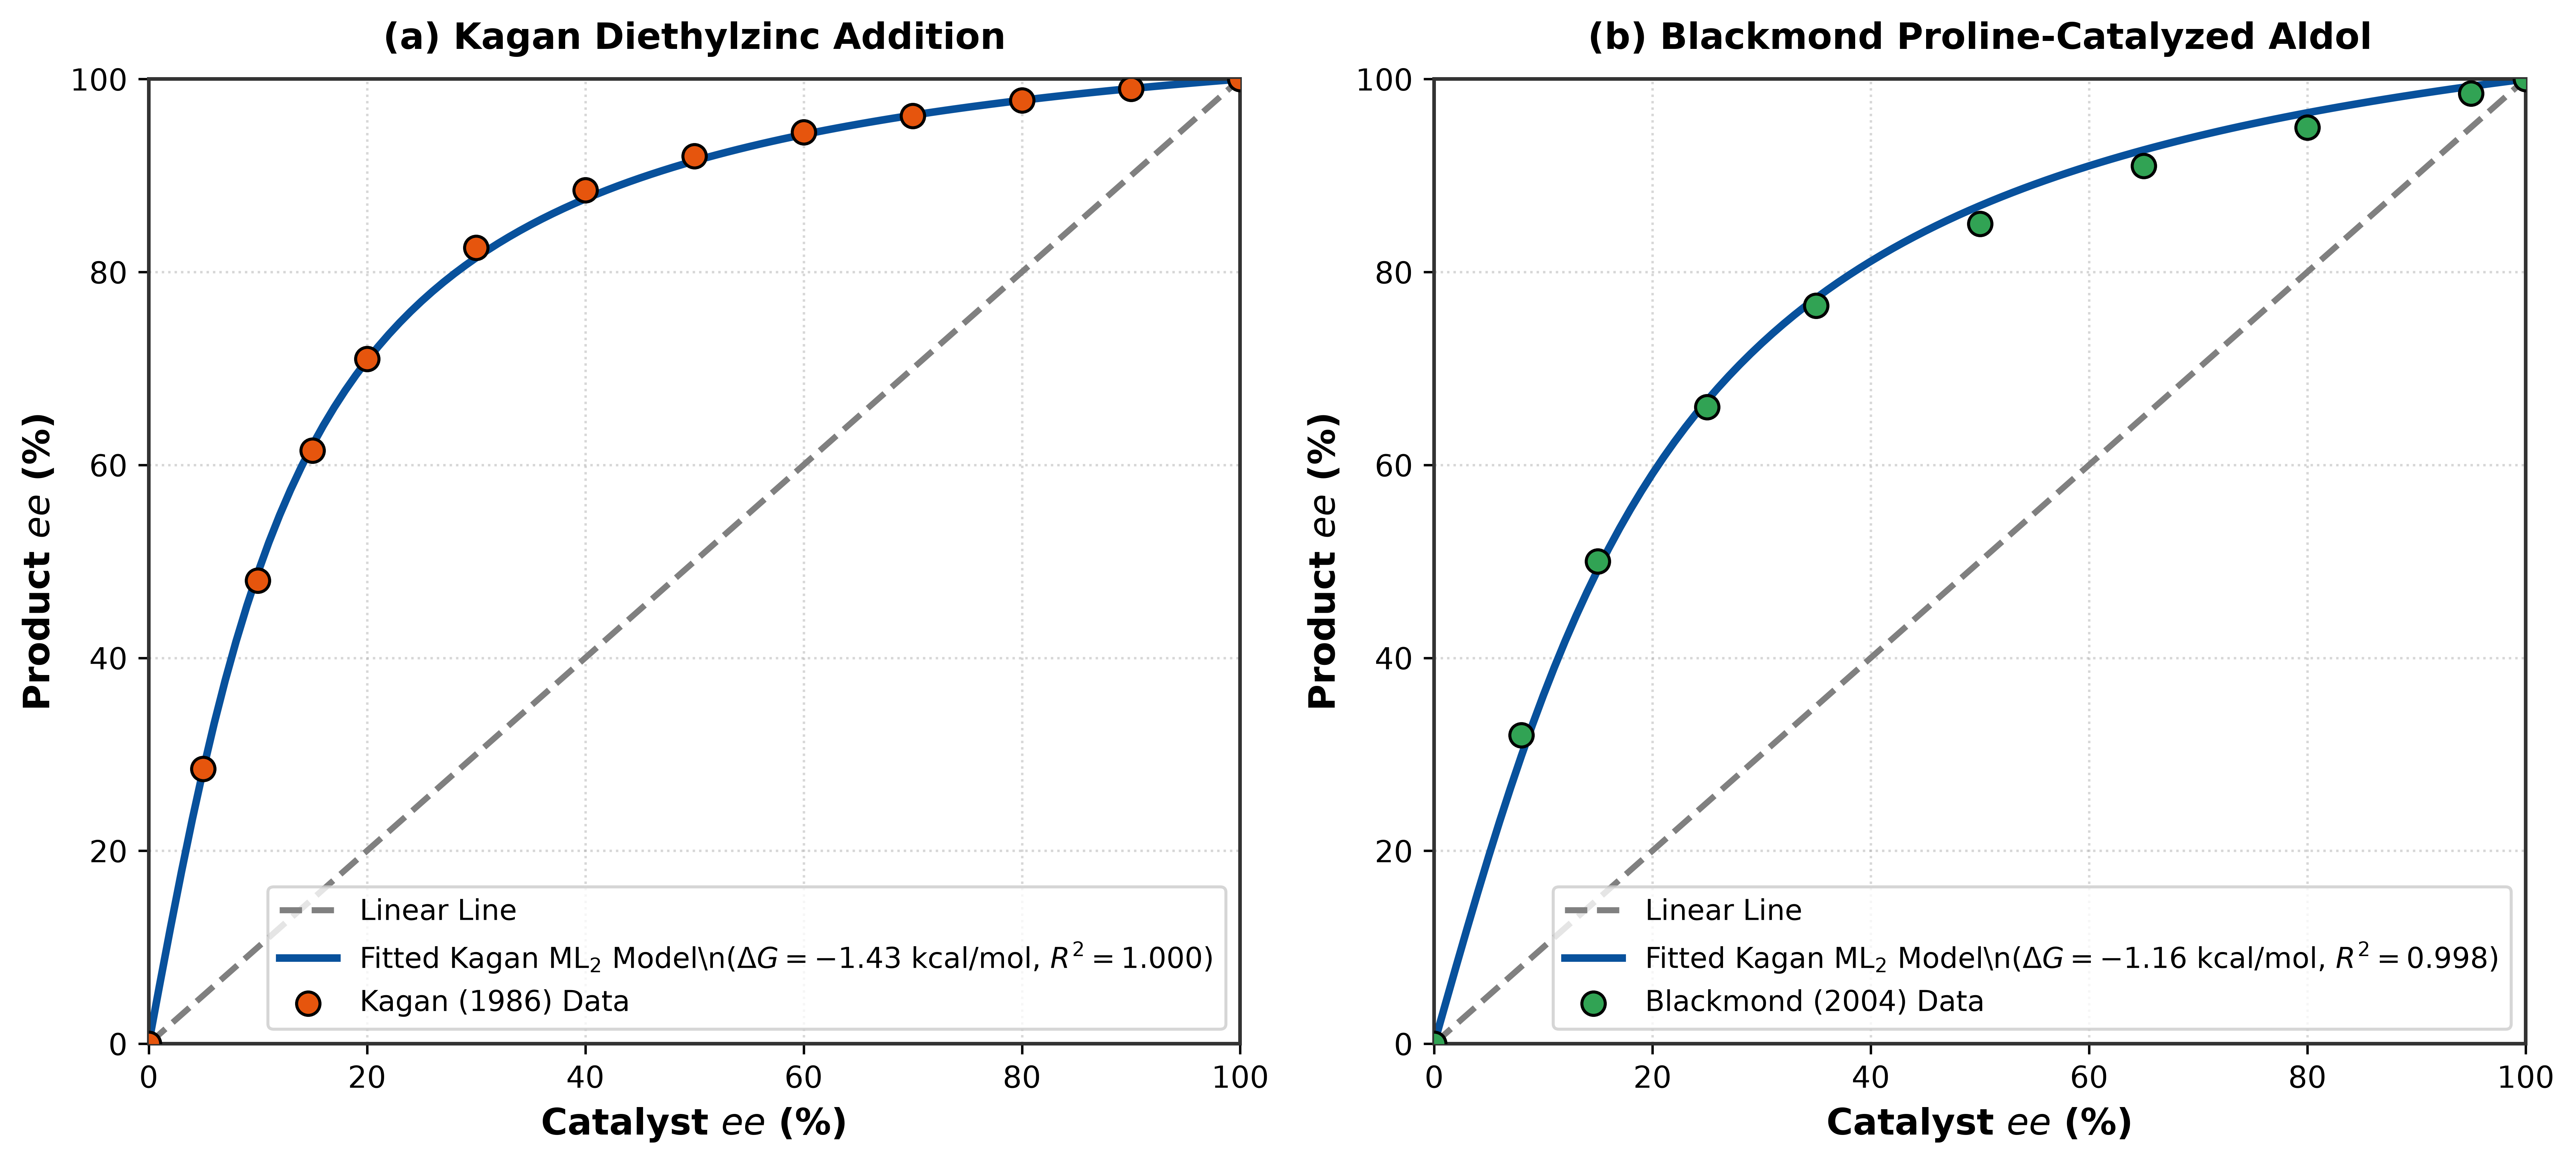
\includegraphics[width=\linewidth]{figures/figure_3_experimental_benchmarks.png}
  \caption{Non-linear parameter estimation and experimental validation for (a) Kagan diethylzinc addition (1986) and (b) Blackmond proline-catalyzed aldol reaction (2004).}
  \label{fig:benchmarks}
\end{figure}

\begin{figure}[htbp]
  \centering
  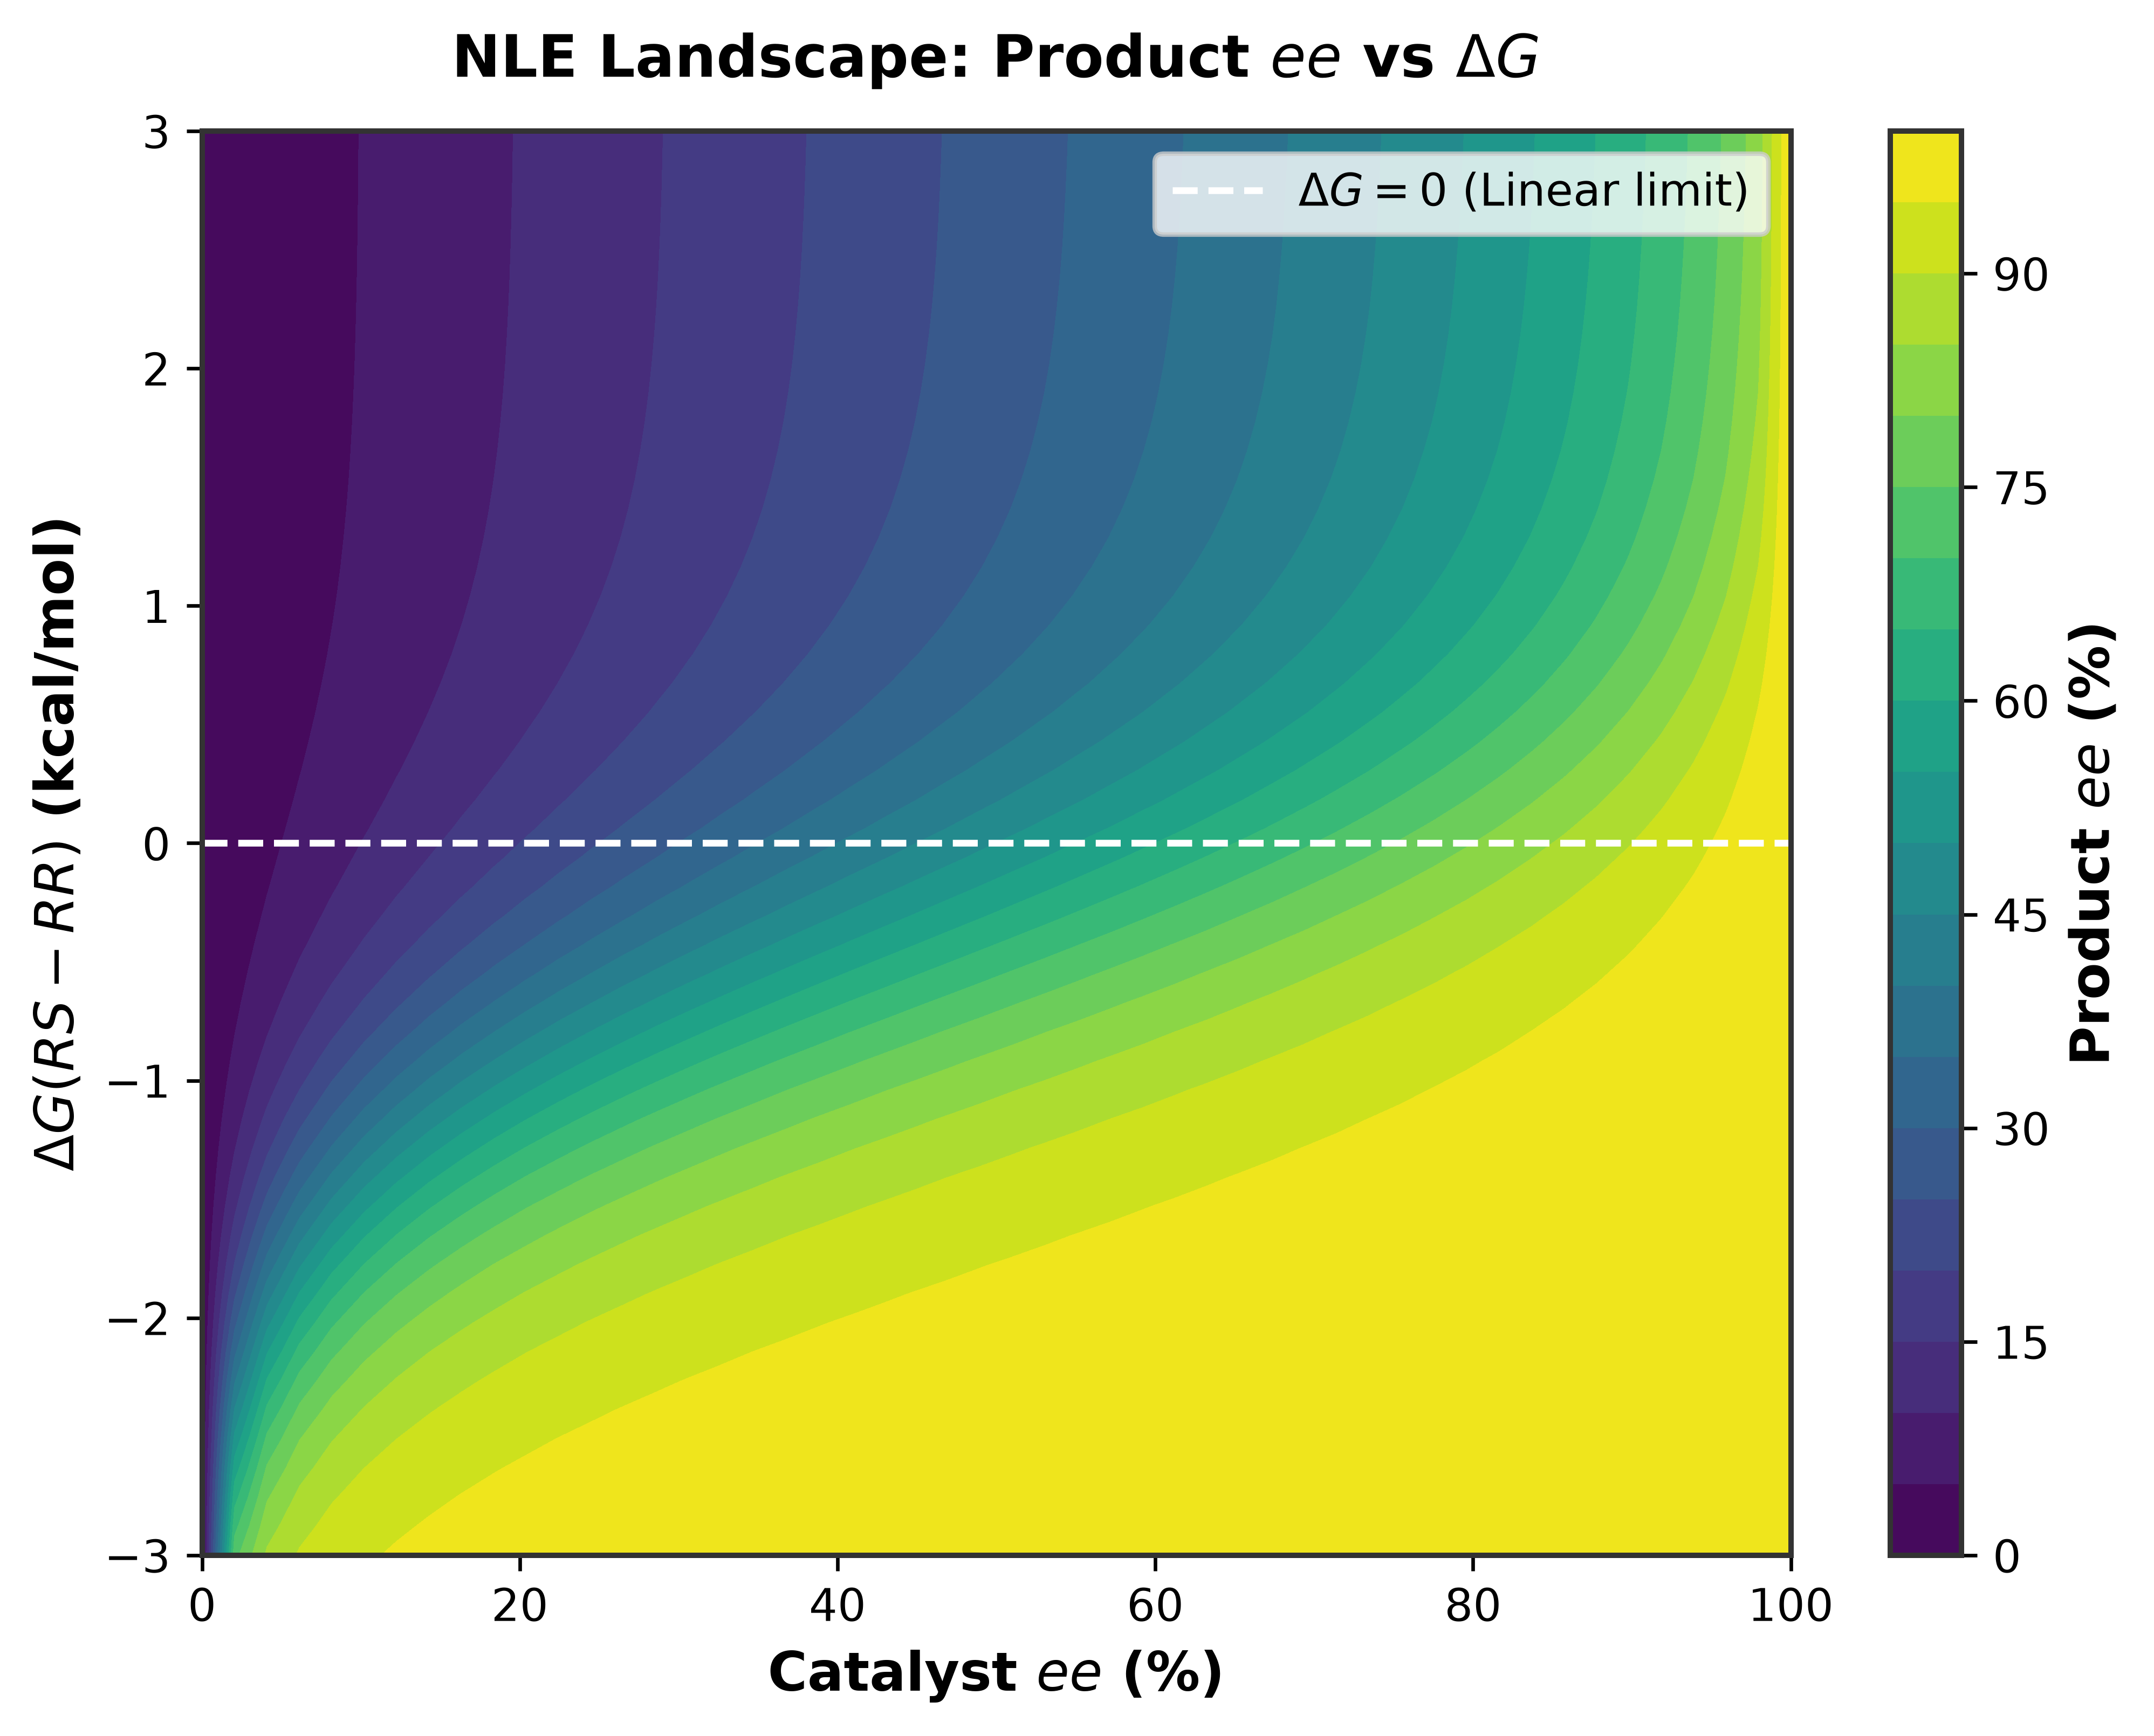
\includegraphics[width=0.75\linewidth]{figures/figure_4_amplification_contour.png}
  \caption{2D amplification contour landscape displaying product enantiopurity as a function of catalyst $ee$ and $\Delta G(RS - RR)$.}
  \label{fig:contour}
\end{figure}

\begin{figure}[htbp]
  \centering
  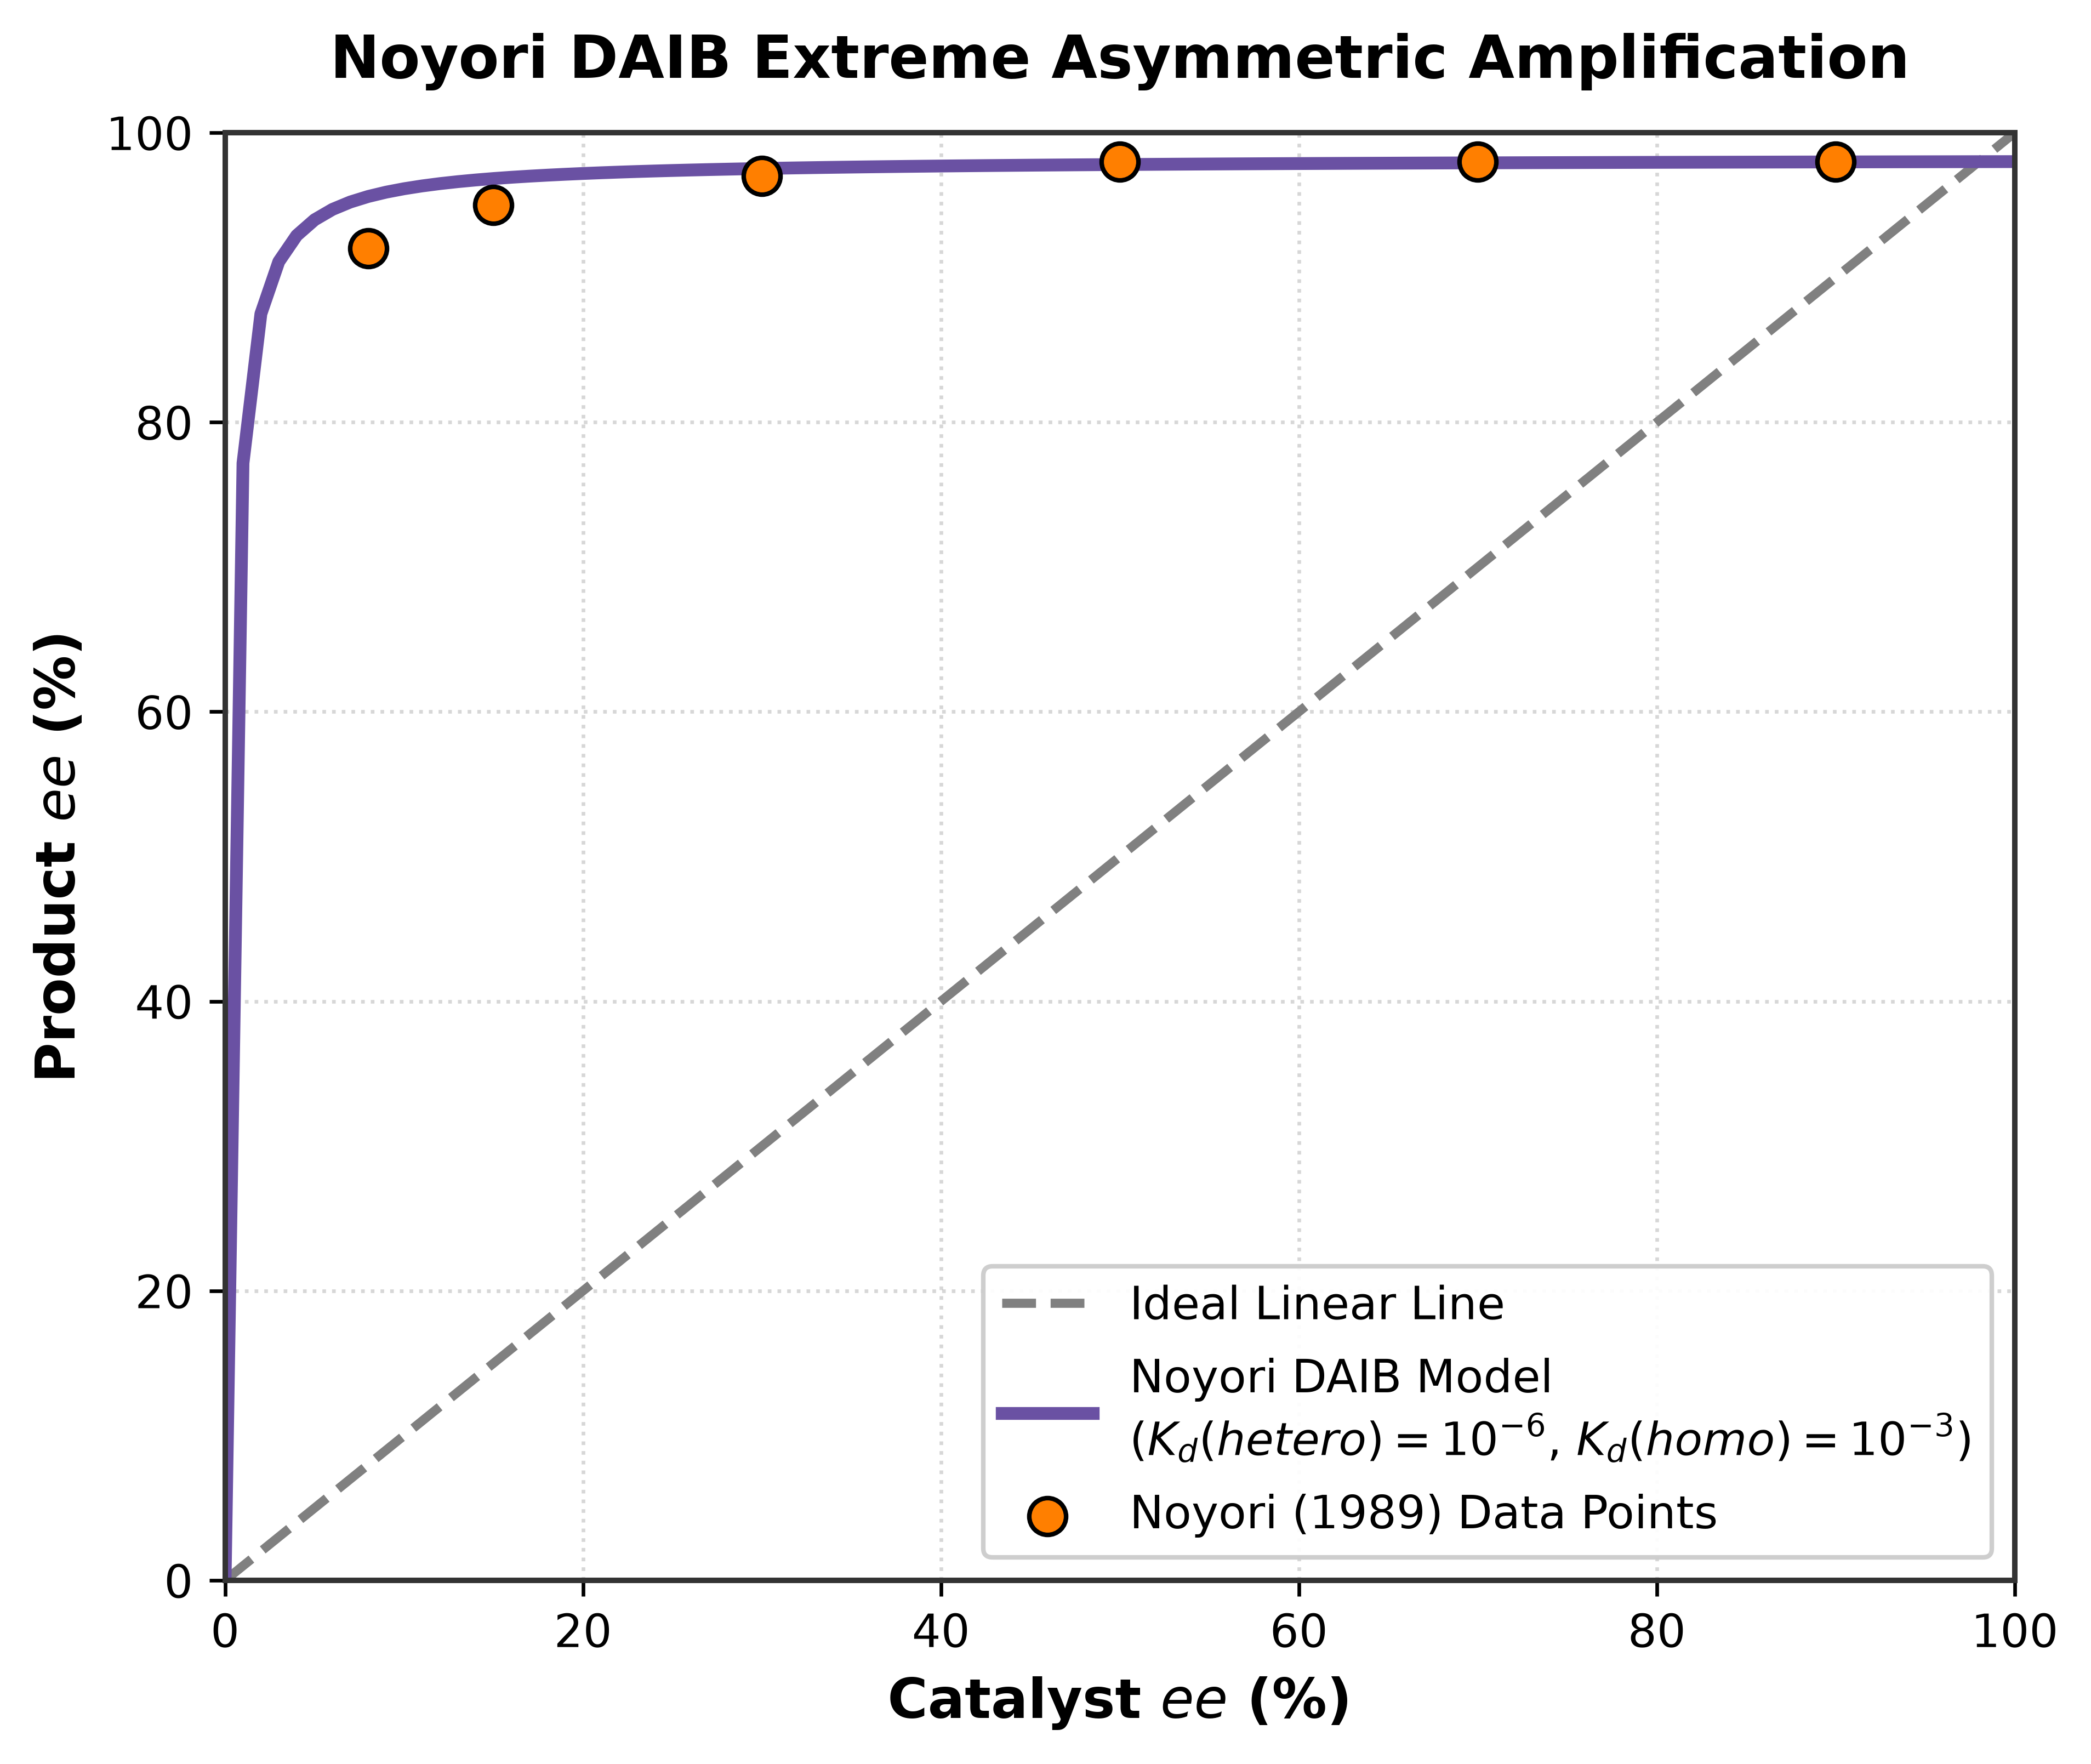
\includegraphics[width=0.75\linewidth]{figures/figure_5_noyori_daib.png}
  \caption{Comparison of the Noyori DAIB aggregation model with experimental measurements from Noyori (1989).}
  \label{fig:noyori}
\end{figure}

\section{Conclusion}
NLE-Predictor bridges the gap between quantum chemical calculations and kinetic modelling of asymmetric catalysis. By resolving numerical stiff-equation bottlenecks with analytical Jacobians and providing robust non-linear parameter estimation, this open-source tool accelerates the design of high-performance chiral catalysts.

\bibliographystyle{unsrt}
\bibliography{references}

\end{document}
